\documentclass{HSECourseW}

\usepackage{graphicx}

% Задаем факультет
\renewcommand{\TitleFaculty}{Факультет компьютерных наук}
\renewcommand{\TitleProgram}{<<Системное программирование>>}
\renewcommand{\TitleDepartment}{программной инженерии}
\renewcommand{\TitleTheme}{Ну прямо очень крутая крутая крутая крутая крутая тема курсовой работы жесть помогите просто я так не могу ахахахахахахах лол кек}
\renewcommand{\TitleGroupNum}{ЫЫТПР1337}
\renewcommand{\TitleAuthor}{Непупкин Василий Григорьевич}
\renewcommand{\TitleSupervisor}{профессор, д.ф.-м.н., Доцент Д. Д.}
\renewcommand{\TitleConsultant}{доцент, к.ф.-м.н., Консультант К. К.}
\renewcommand{\TitleCity}{Москва}
\renewcommand{\TitleYear}{2025}


\begin{document}

\titlepage

\begin{abstractpage}
	Тестируем аннотацию. Курсовая работа представляет собой одну из форм самостоятельной научно-исследовательской работы студентов, направленную на углубление теоретических знаний и развитие практических навыков по изучаемой дисциплине. В процессе выполнения работы студент должен продемонстрировать умение анализировать литературные источники, формулировать цели и задачи исследования, применять соответствующие методы и средства для достижения поставленных целей, а также обобщать полученные результаты и делать выводы. 
	
\end{abstractpage}

\tableofcontents

\section{Введение}  

Курсовая работа представляет собой одну из форм самостоятельной научно-исследовательской работы студентов, направленную на углубление теоретических знаний и развитие практических навыков по изучаемой дисциплине. В процессе выполнения работы студент должен продемонстрировать умение анализировать литературные источники, формулировать цели и задачи исследования, применять соответствующие методы и средства для достижения поставленных целей, а также обобщать полученные результаты и делать выводы.  \cite{ispras}

\begin{figure}[htbp]
	\centering % Центрирование
	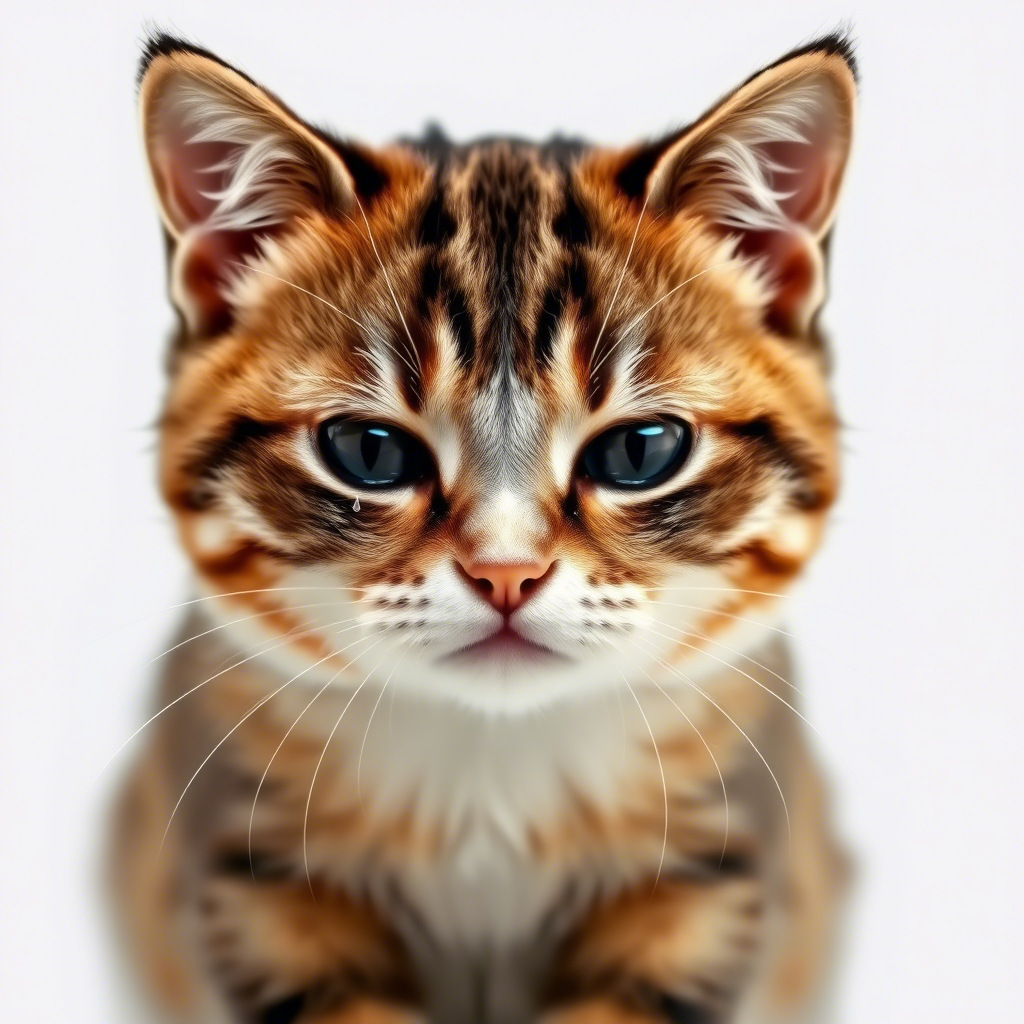
\includegraphics[width=0.5\textwidth]{crycattest.png} % Путь к файлу
	\caption{Тестируем подпись к рисунку} % Подпись
	\label{fig:crycattest} % Метка для ссылок
\end{figure}

Современный этап развития информационных технологий предъявляет всё более высокие требования к уровню подготовки специалистов в области компьютерных наук и инженерии программного обеспечения. В связи с этим выполнение курсовых работ становится важным элементом образовательного процесса, способствующим не только закреплению знаний, но и развитию исследовательских навыков, необходимых для последующего написания выпускной квалификационной работы. 

\section{Цель и задачи работы}  

\subsection{Основная цель}
Основной целью курсовой работы является систематизация, закрепление и расширение теоретических и практических знаний студента по избранной теме.
\begin{figure}[htbp]
	\centering % Центрирование
	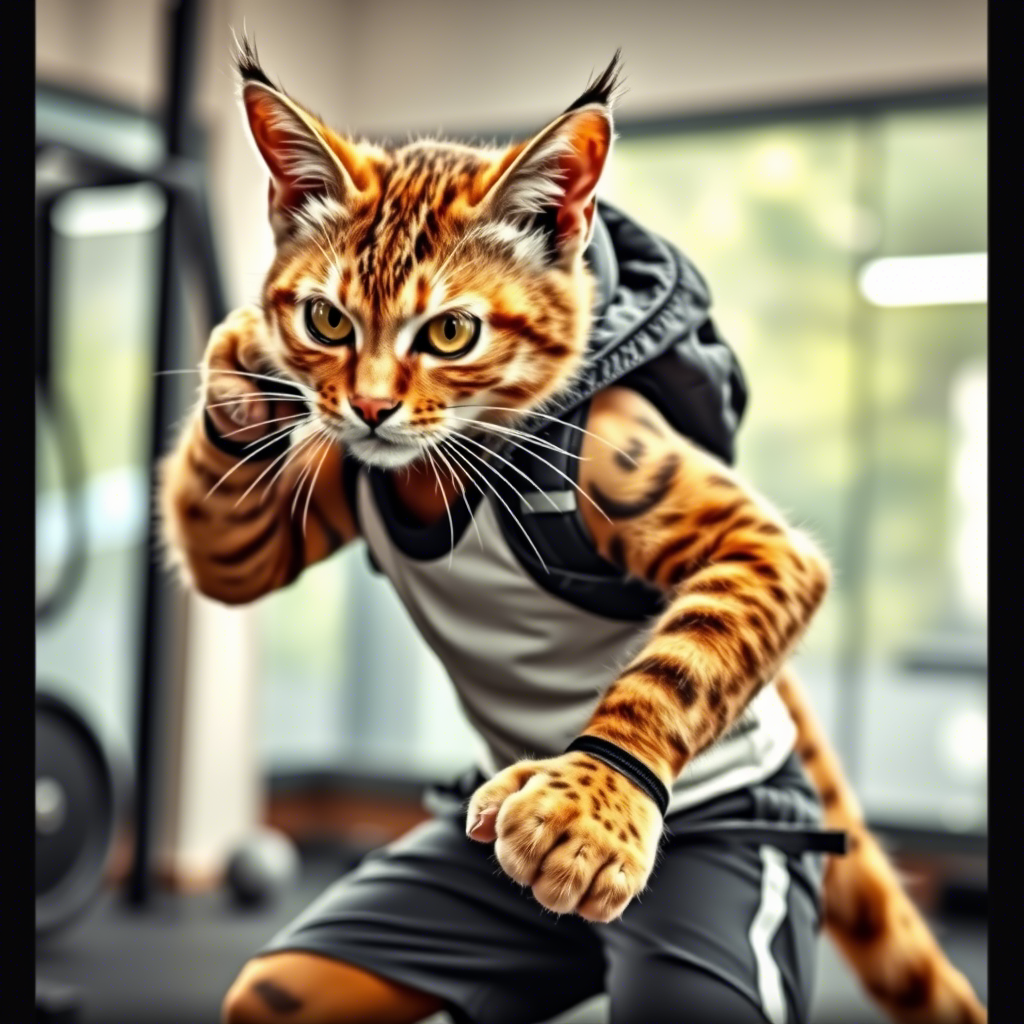
\includegraphics[width=0.5\textwidth]{sportcat.png} % Путь к файлу
	\caption{Тестируем подпись к рисунку} % Подпись
	\label{fig:sportcat} % Метка для ссылок
\end{figure}
Для достижения этой цели ставятся следующие задачи: изучить современное состояние проблемы; провести анализ существующих подходов и методов решения; выбрать наиболее эффективный метод или разработать собственный алгоритм; реализовать прототип системы или программного модуля; провести тестирование и оценку качества разработанного решения; оформить результаты исследования в соответствии с установленными нормами и стандартами. 

\subsection{Актуальность выбранной темы}
Актуальность выбранной темы определяется тем, что она находится на пересечении нескольких областей знаний, таких как искусственный интеллект, машинное обучение и обработка больших данных. Это позволяет не только применять современные технологии для решения конкретной задачи, но и развивать навыки работы с реальными данными, а также использовать инструменты автоматизации анализа информации. 



\section{Методология и методы исследования}  

Для достижения поставленных целей использовались как теоретические, так и практические методы исследования. К теоретическим относится анализ научной литературы и изучение современных подходов к решению аналогичных задач. Практическая часть включает в себя разработку программного обеспечения, проведение вычислительных экспериментов и анализ полученных результатов. 

Одним из ключевых этапов работы стал выбор модели машинного обучения, которая должна была обеспечить высокую точность прогнозирования при минимальных вычислительных затратах. Было проведено сравнение нескольких популярных алгоритмов, таких как логистическая регрессия, деревья решений, случайный лес и нейронные сети. Окончательный выбор был сделан на основе результатов тестирования на наборе данных, взятом из открытых источников. 

После реализации модели был проведён анализ её поведения на различных типах входных данных. Также были разработаны рекомендации по её дальнейшему улучшению и возможностям применения в других задачах. 

% СПИСОК ЛИТЕРАТУРЫ....
\bibliographystyle{gost71u} % Для соответствия требованиям об оформлении списка литературы
\bibliography{references}

\end{document}